%!TEX root = thesis.tex

% a related work section in which the relevant literature is presented and linked to the project;
% ~15 pages 

\chapter{Related work}
\label{chap:rw}
A number of research topics are relevant for this thesis: how to use existing standards for publishing sensor data to the semantic web, developing ontologies that are suitable for many different kinds of sensor data and how to aggregate sensor data based on geographical features and time. This chapter discusses the recent relevant literature on these topics.  

\section{Sensor data catalogue service}
The \ac{ogc} has developed a way of including sensors into a registry.

\begin{figure}
	\centering
	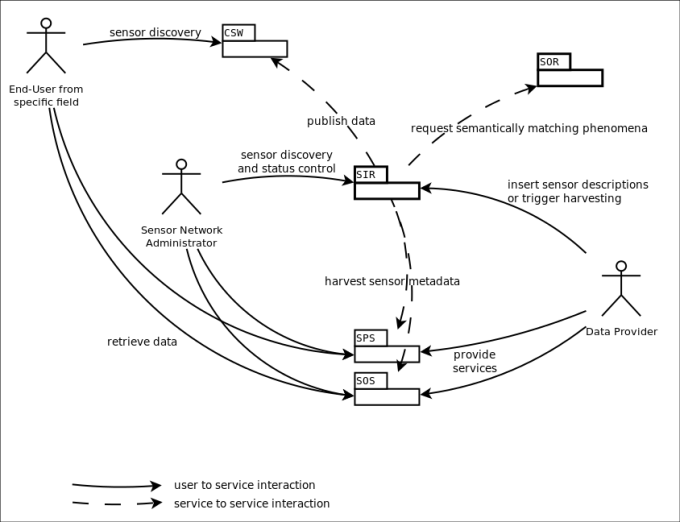
\includegraphics[width=0.6\linewidth]{figs/sor_sir.png}
	\caption{Overview of the interaction between SIR, SOR and potential users. By \cite{SW:52North2}}
	\label{fig:SorSir}
\end{figure}

\subsection{Sensor observable registry}
The \ac{sor} is \enquote{a web service interface for managing the definitions of phenomena measured by sensors as well as exploring semantic relationships between these phenomena} \cite[p. vi]{SW:OGC4}. This is a web service developed by \ac{ogc} to enable semantic reasoning on sensor networks, especially concerning phenomenon definitions. This should make it easier to discover sensors that observe a certain phenomenon and to interpret sensor data.

The \ac{sor} has four different requests: \texttt{GetCapabilities}, \texttt{GetDefinition-} \texttt{URNs}, \texttt{GetDefinition} and \texttt{GetMatchingDefinitions}. The \texttt{GetCapabilities} request provides an overview of what the \ac{sor} has to offer. The capabilities document that is returned to the client contains four sections. The service identification section lists general information about the service, such as the title and supported \ac{sor} versions, but also whether there are fees or access constraints. The service provider section contains details on which organisation provides the \ac{sos} and lists their contact information. The operations metadata section lists the supported request types. These sections are required for every \ac{ogc} geoweb service. The fourth section is the content section. This part of the capabilities document contains the following information: the number of entries inside the \ac{sor} instance, keywords describing the content of the \ac{sor} instance, the application domain for which a specific \ac{sor} can be applied and an `ontologyRepositoryURL'. This \ac{url} points to a repository that contains an ontology used by this \ac{sor}.

\texttt{GetDefinitionURNs} returns a list of \acp{urn} identifying the definitions that are present in the \ac{sor}. Optionally a client can add a `SearchSensor' parameter to filter \acp{urn}. This parameter takes a substring that shall occur within the definition \acp{urn} to be returned. Also, a maximum limit for the amount of returned \acp{urn} can be added using the `maxNumberOfResults' parameter. The optional parameter `startResultElement' can be used to input the number of the first returned result element.

For retrieving the definition of a specific \ac{urn} a \texttt{GetDefinition} request can be made. This request takes an \ac{urn} of the phenomenon for which a definition should be retrieved as input. The definition is returned as a GML dictionary entry.  

\texttt{GetMatchingDefinitions} allows clients to retrieve definitions of observables which in some way are related to another given phenomenon. The relations `generalization', `specialization' and `equivalency' are currently supported for finding matching definitions \citep{SW:OGC4}.   

\subsection{Sensor instance registry}
Another web service interface specification by \ac{ogc} is \ac{sir}. \ac{sir} is aimed at \enquote{managing the metadata and status information of sensors} \cite[p. xii]{SW:OGC3}. The goal of this web service is to close the gap between metadata models based on \ac{sensorml}, which is used in \ac{swe}, and the metadata model used in \ac{ogc} catalogue services. Furthermore, it provides functionalities to discover sensors, to harvest sensor metadata from a \ac{sos}, to handle status information about sensors and to link \ac{sir} instances to \ac{ogc} catalogue services. 

\begin{sloppypar}
There are 14 different requests that can be made at a \ac{sir}. First of all, there is the \texttt{GetCapabilities} request, which provides an overview of what the service has to offer. For searching and retrieving sensor metadata there are the \texttt{SearchSensor} and \texttt{DescribeSensor} requests. 

The \texttt{HavestService} request allows to retrieve all metadata from an \ac{swe} service. 

Transactions for individual sensors can be made using \texttt{InsertSensorInfo}, \texttt{DeleteSensorInfo}  and \texttt{UpdateSensorDescription}. 

Sensor status information can be managed using \texttt{GetSensorStatus}, \texttt{SubscribeSensorStatus}, \texttt{RenewSensorStatusSubscription}, \texttt{CancelSensorStatusSubscription} and \texttt{InsertSensorStatus}. 

Managing the connection between a \ac{sir} and a \ac{ogc} catalog can be done using \texttt{ConnectToCatalog} and \texttt{DisconnectFromCatalog} requests \citep{SW:OGC3}.
\end{sloppypar}

\section{Semantic sensor data middleware}
\cite{SSW:Henson} and \cite{SSW:Pschorr} suggest adding semantic annotations to a \ac{sos} which they call \ac{semsos}. In \ac{semsos} the raw sensor data goes through a process of semantic annotating before it can be requested with a \ac{sos} service. The retrieved data is still an \ac{xml} document, but with embedded semantic terminology as defined in an ontology. The data retrieved from \ac{semsos} is therefore semantically enriched.  

\cite{SSW:Pschorr2} has created a prototype that is able to find sensors from a \ac{sos} using linked data. The user can input a location and find sensors that are located nearby. They acknowledge the advantages of linked data over a catalogue service. However, the method presented by \cite{SSW:Pschorr2} is still limited to retrieving sensors from a single source in a buffer around a point location.  

\cite{SSW:Janowicz} has specified a method that uses a \ac{rest}ful proxy as a fa\c{c}ade for \ac{sos}. When a specific \ac{uri} is requested the so-called \ac{sel} translates this to a \ac{sos} request, fetches the data and translates the results back to \ac{rdf}. In this method the sensor data is converted to \ac{rdf} on-the-fly. This allows the data to be interpreted by both humans and machines.  

\cite{SSW:Atkinson} have identified that \enquote{distributed heterogeneous data sources are a necessary reality in the case of widespread phenomena with multiple stakeholder perspectives} \cite[p.129]{SSW:Atkinson}. Therefore, they propose that methods should be developed to move away from the traditional dataset centric approaches and towards using linked data for cataloguing. This has the potential to bring together data and knowledge from different areas of research about the same (or similar) features-of-interest. It is also argued that using both linked data services and data-specific services could ease the transition into the linked data world.  

\section{Sensor data ontologies}

Ontologies are necessary to provide meaning to data on the semantic web and to create semantic interoperability. Three recent efforts for developing a standard ontology for sensor data based on \ac{swe} standards will be discussed here.

\subsection{Semantic sensor network ontology} 
\ac{w3c} has developed an ontology for sensors and observations called the \ac{ssno}. This ontology aims to address semantic interoperability on top of the syntactic operability that the \ac{swe} standards provide. To accommodate different definitions of the same concepts the broadest definitions have been used. Depending on the interpretation these can be further defined with subconcepts. The \ac{ssno} is based on the stimulus-sensor-observation pattern, describing the relations between a sensor, a stimulus and observations (Figure \ref{fig:sens-stim-obs}). Sensors are defined as \enquote{physical objects ... that observe, transforming incoming stimuli ... into another, often digital, representation}, stimuli are defined as \enquote{changes or states ... in an environment that a sensor can detect and use to measure a property} and observations are defined as \enquote{contexts for interpreting incoming stimuli and fixing parameters such as time and location} \cite[p. 28]{SSW:SSN_incubatorGroup}. The ontology can be used to model sensor networks from four different perspectives (sensor, observation, system, and feature \& property), which they discuss together with additional relevant concepts.

\begin{figure}
	\centering
	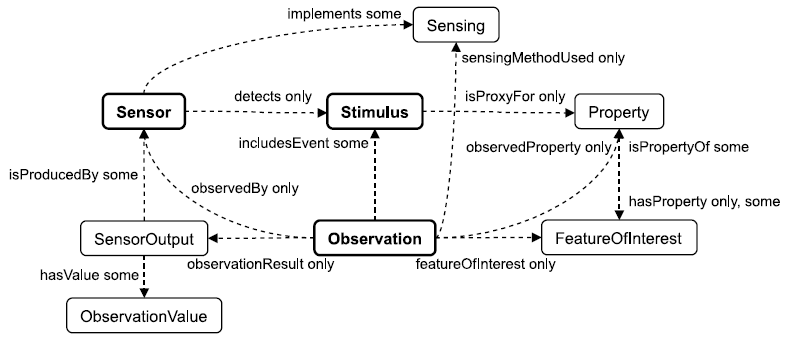
\includegraphics[width=1\linewidth]{figs/sens_stim_obs.png}
	\caption{The stimulus–sensor–observation pattern \cite[p. 28]{SSW:SSN_incubatorGroup}}
	\label{fig:sens-stim-obs}
\end{figure}

\subsection{Observation capability metadata model} 
\cite{SW:Hu} have reviewed a number of metadata models (including \ac{sensorml} and \ac{ssno}) for the use of earth observation (including remote sensing). They argue that all of the current metadata models are not sufficient for sensor data discovery. This conclusion is based on an evaluation of six criteria. Three steps were identified in the process of obtaining relevant sensor data for earth observation, which have been used to derive criteria for their evaluation framework. These steps are sensor filtration, sensor optimisation and sensor dispatch. The filtration of sensors should result in a set of sensors that meets the requirements of the application: It should measure the right phenomenon, be active, be inside the spatial and temporal range, and have a certain sample interval. In sensor optimisation the selected sensors should be combined to complement or enhance each other. To do this, the observation quality, coverage and application is relevant. In the last step -- sensor dispatch -- the data should be retrieved, stored and transmitted. In every evaluated model the same sensors can be described in different ways or only partially, which affects the outcome of the sensor dispatch. 

Therefore, a metadata model is proposed that \enquote{reuses and extends the existing sensor observation-related metadata standards} \cite[p. 10546]{SW:Hu}. It is composed of five modules: observation breadth, observation depth, observation frequency, observation quality and observation data. They should be derived from metadata elements described using the Dublin Core metadata element set. These five modules can then be formalised following the \ac{sensorml} schema which can be queried by users via a `Unified Sensor Capability Description Model-based Engine'. 

\subsection{Om-lite \& sam-lite ontologies}
\cite{SSW:Cox4} has been working on new semantic ontologies based on \ac{om}. Previous efforts, such as the \ac{ssno} have been using pre-existing ontologies and frameworks. However, there are already many linked data ontologies that could be useful for describing observation metadata, such as space and time concepts. Also, the \ac{ssno} does not take sampling features into account. Therefore, \cite{SSW:Cox4} proposes two new ontologies: \ac{owl} for observations or om-lite \citep{SSW:Cox3}, which defines the concepts from \ac{om} regarding observations and \ac{owl} for sampling features or sam-lite, which defines the sampling feature concepts \citep{SSW:Cox2}. A mapping of the \ac{ssno} to om-lite is also provided.

\cite{SSW:Cox4} describes how the PROV ontology \citep{LD:PROV} can be directly used inside om-lite. The PROV ontology is \enquote{concerned with the production and transformation of Entities through time-bounded Activities, under the influence or control of Agents} \cite[p. 12]{SSW:Cox4}. This is a very convenient ontology for modelling real world entities, such as sensors, observation processes and sampling processes. Many other ontologies could be implemented in combination with om-lite and sam-lite, depending on the kind of observations that are being modelled and the data publisher's preference. 

\section{Sensor data aggregation}
Sensor data aggregation can be performed for two purposes: To reduce the energy constraint of sensor networks \citep{SW:Korteweg} or to sample a feature-of-interest in space and/or time \citep{SDI:INSPIRE2}. Sampling is performed when a feature-of-interest is not accessible, in which case \enquote{observations are made on a subset of the complete feature, with the intention that the sample represents the whole} \citep{SSW:Cox3}. \cite{SSW:Stasch3} proposes a \ac{wps} that retrieves sensor data from a \ac{sos} service in order to aggregate it based on features-of-interest. The approach by \cite{SSW:Stasch} is similar, but takes sensor data as input that is already published on the semantic web.

\cite{SW:Ganesan} stresses that spatio-temporal irregularities are fundamental to sensor networks. Irregular sampling can have a potentially large influence on the accuracy of the aggregated outcome. For example, averaging sensor data from a feature-of-interest that is being sampled densely in some parts and more sparsely in other parts could lead to inaccurate results. To counter this the values of the densely sampled area should have a lower weight than the values from the sparsely sampled area. The same holds true for temporal irregularities \citep{SW:Ganesan}. Also, \cite{SSW:Stasch4} argue that in order for automatic aggregation to work there needs to be semantics on which kind of aggregation methods are appropriate for a specific kind of sensor data. Not all kinds of aggregation are meaningful (e.g. taking the sum of temperature values). This requires a formalisation of expert knowledge which they call semantic reference systems. 




